
\chapter{Motivation}
\section{Inspiration}
Inspired by the movie \textit{2001: A Space Odyssey} produced and directed by Stanley Kubrick, an adaption has been created by using povray. The adaption contains selected scenes of 5 minute clip on youtube.  With the exception of few scenes the cuts and scenes as well as the soundtrack are geared to the original video  \cite{EbClectic}.

\chapter{Models}
The whole short animation is created has been written and created in povray. Everything but the starships (section \ref{imported_models}) has been created from scratch without using any tools.

\section{Imported Models} \label{imported_models}

We found the models of the Orion III Spaceplane and Space Station V by B.J. West with Textures by Michael Powell in the 2001: A Space Odyssey 3D Modelling Archiv \cite{Archive}.
Since both models were not available in a format directly usable with POV-Ray but \textit{3ds Max} (former called \textit{3D Studio Max}), we had to convert them from Autodesks proprietary format (.max) to the open Wavefront .obj format, which we then converted to POV-Ray code using PoseRay \cite{PoseRay}.

\section{Remarkable Models}
\subsection{Human} \label{human_model}
\subsection{Cabin} 
\newpage
\subsection{Cockpit} \label{cockpit_model}
Inspired by the cockpit (figure \ref{cockpit_original}) shown in the movie, the cockpit in the adaption  is built completely from scratch using povray (figure \ref{cockpit_povray}). The starship \textit{Station} on this scene belongs to the imported models (section \ref{imported_models}). 
The pilots are transformed models of the human \ref{human_model}. 
\begin{figure}[ht]
	\centering
	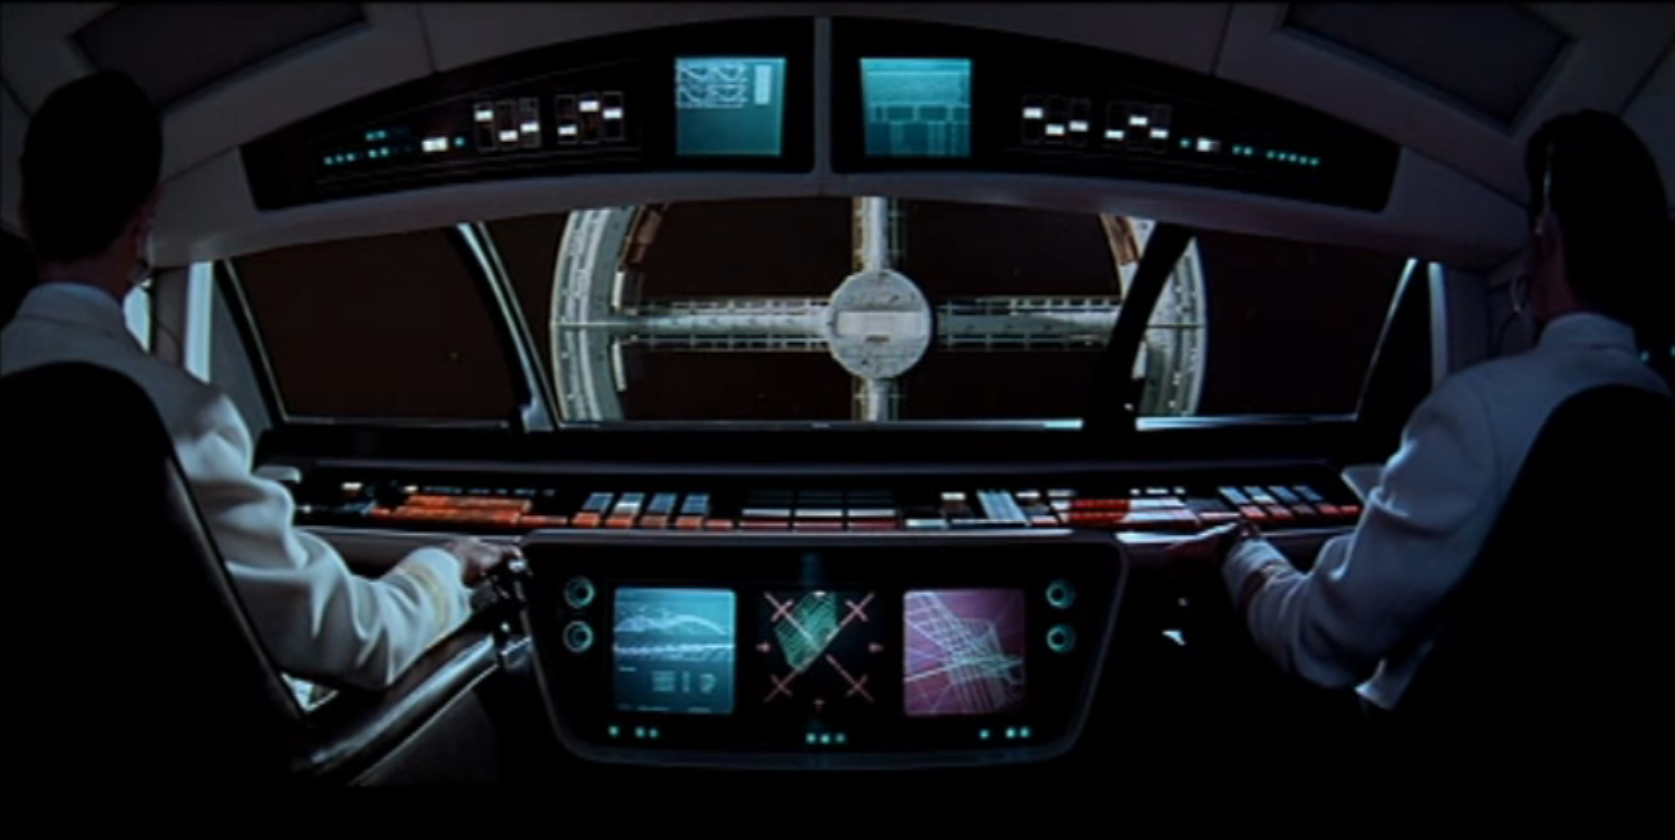
\includegraphics[width=0.8\textwidth]{images/original_cockpit_scene19.png}
	\caption{Cockpit of Starship \textit{Orion} taken from \textit{2001: A Space Odyssey}}
	\label{cockpit_original}
\end{figure}

\begin{figure}[ht]
	\centering
	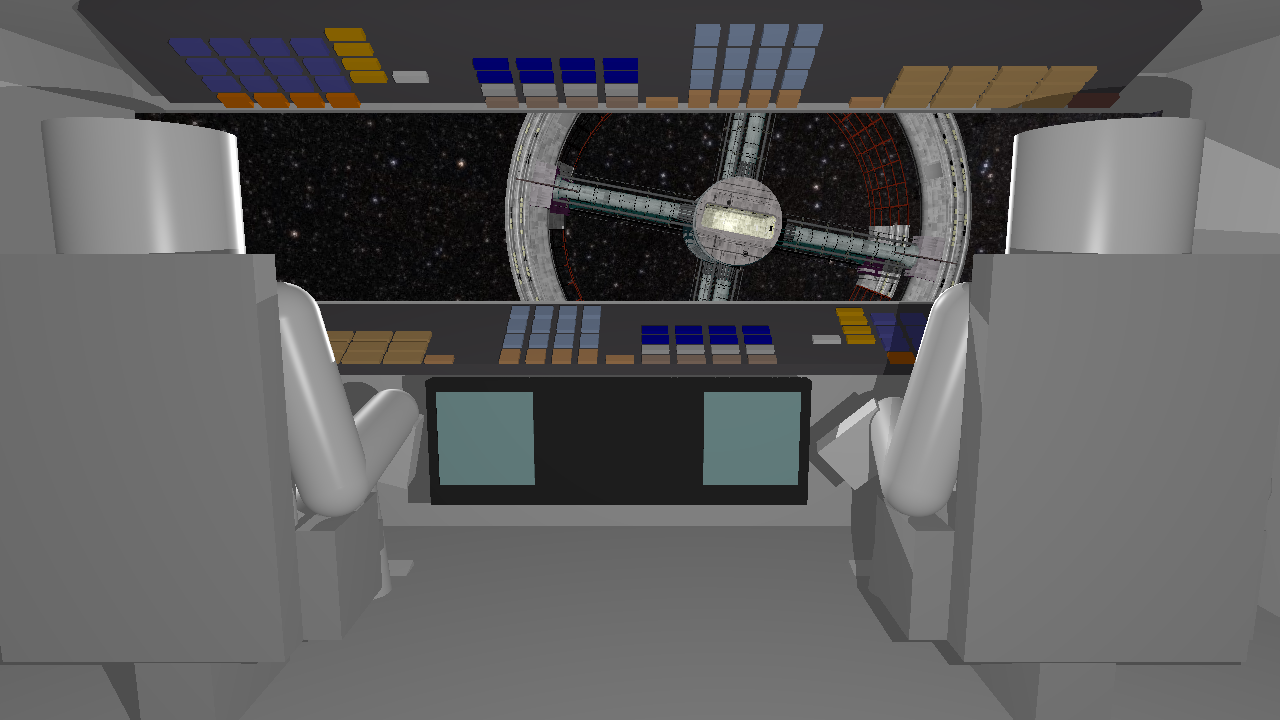
\includegraphics[width=0.8\textwidth]{images/scene19587.png}
	\caption{Cockpit of Starship \textit{Orion} built in povray.}
	\label{cockpit_povray}
\end{figure}

The associated povray script can be found on GitHub \cite{Quving}.

\newpage
\subsection{Earth}

\chapter{Production}
\section{Rendering}
\section{Post-Production}
